\documentclass{article}
\usepackage{amsmath}
\usepackage{graphicx}

\begin{document}
\begin{center}
    \huge\bfseries Reeksamen 2015 - Februar \\
\end{center}
Opgave 3 (21\%) \\

\noindent
$a)$ Lad $R$, $S$, og $T$ være binære relationer på mængden $\{1,2,3,4\}$.
\begin{align*}
    R &= \{(1,1),(2,1),(2,2),(2,4),(3,1),(3,3),(3,4),(4,1),(4,4)\}
\end{align*}
Er $R$ en partiel ordning?

For at $R$ skal være en partiel ordning, skal den opfylde tre krav:
\begin{enumerate}
    \item Refleksivitet: Hvert element er relateret til sig selv. Alle elementer er relateret til sig selv, da vi har 4 unikke elementer: $(1,1)$, $(2,2)$, $(3,3)$ og $(4,4)$.
    
    \item Antisymmetri: Der må ikke være to forskellige elementer, der er indbyrdes relaterede begge veje. Der findes ikke et par som f.eks. $(1,2)$ og $(2,1)$, hvilket ville gøre det symmetrisk. Dette gælder også for de resterende elementer: $(2,4)$, $(3,1)$, $(3,4)$ og $(4,1)$.
    
    \item Transitivitet: Hvis to elementer er relateret på en bestemt måde, og et tredje element er relateret til det andet, så skal det første element også være relateret til det tredje. Dette ses for: $(2,1)$, $(2,2)$ og $(2,4)$. Dette gælder også for andre elementer i $R$.
\end{enumerate}
$R$ opfylder alle krav til at være en partiel ordning. \\
\newpage
$b)$ Lad $S = \{(1,2),(2,3),(2,4),(4,2)\}$.
Angiv den transitive lukning af $S$. \\
\begin{figure}[h!]
    \centering
    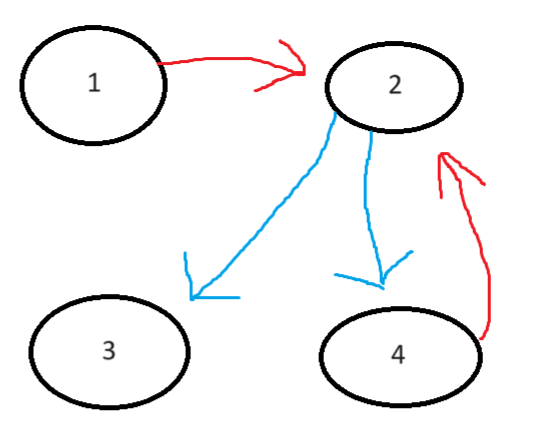
\includegraphics[width=7cm]{Pictures/123123123123.png}
    \caption{En visualisering af den transitive lukning af S}
    \label{fig:S}
\end{figure}

Den transitive lukning af $S$ er:
\begin{align*}
    S_{\text{lukket}} &= \{(1,2),(1,3),(1,4),(2,1),(2,3),(2,4), \\
    &\quad (3,1),(3,2),(3,4),(4,1),(4,2),(4,3)\}
\end{align*}

\noindent
$c)$ Lad $T=\{(1,1),(1,3),(2,2),(2,4),(3,1),(3,3),(4,2),(4,4)\}$.
Bemærk, at $T$ er en ækvivalensrelation.
Angiv $T$'s ækvivalensklasser. \\

\noindent
Ækvivalensklasse 1: $\{1,3\}$ \\
Ækvivalensklasse 2: $\{2,4\}$

\newpage
\end{document}